\documentclass{standalone}
\usepackage{pgfplots}
\pgfplotsset{
  compat=1.18, 
  trig format=rad, 
  ticklabel style = {font=\footnotesize},
}

\begin{document}
  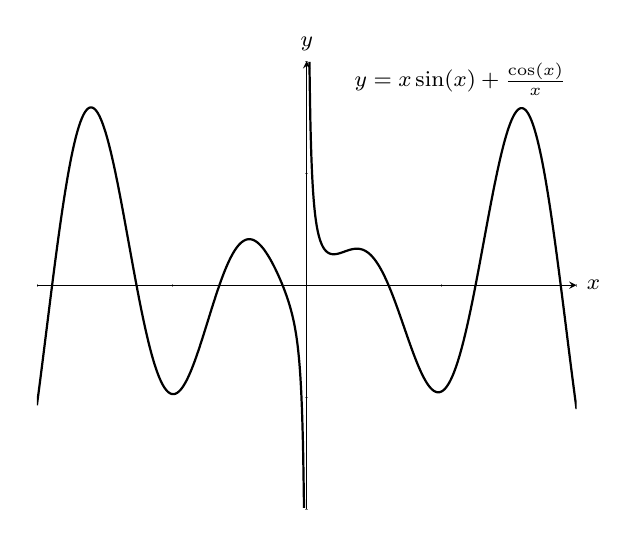
\begin{tikzpicture}
    \begin{axis}[
      axis lines=middle,
      ymin=-10, ymax=10,
      xmin=-10, xmax=10,
      xlabel={\footnotesize \(x\)},
      xlabel style={at={(ticklabel* cs:1)}, anchor=west},
      ylabel={\footnotesize \(y\)},
      ylabel style={at={(ticklabel* cs:1)}, anchor=south},
      axis line style = {very thin},
      yticklabels={,,},
      xticklabels={,,},
      smooth,
      thick,
      no markers,
      tickwidth={1pt},
      samples=300,
      ]
      \addplot[smooth, domain=0.1:10] {x*sin(x)+cos(x)/x};
      \addplot[smooth, domain=-10:-0.1] {x*sin(x)+cos(x)/x};
      \node[above left] at (10,8) {\footnotesize \(y = x\sin(x) + \frac{\cos(x)}{x}\)};
    \end{axis}
  \end{tikzpicture}
\end{document}
